\Exercise{Eine einfache Canvas Animation}
%
\par Entwerfen Sie eine HTML Seite, die ein \htag{canvas}-Element sowie drei
Buttons (Langsamer, Schneller, Abspielen / Pause) beinhaltet. Über den Button
Abspielen soll eine Animation (in Dauerschleife) gestartet werden. Beim
erneuten Klick auf den Button soll die Animation angehalten werden.
%
\par Gehen Sie am besten folgendermaßen vor:
%
\begin{itemize}
\item
Erstellen Sie eine \jfunc{drawCanvas}-Methode, die mit dem entsprechenden
Kontext Zeichnungen durchführt.
\item
Beim Klicken auf den Startbutton soll über \jfunc{setInterval} ein gepulster
Timer erstellt werden, der in regelmäßigen Abständen die
\jfunc{drawCanvas}-Methode ausführt.
\item
Beim erneuten Klick auf den Startbutton soll der Timer über
\jfunc{clearInterval} gelöscht werden.
\item
Schneller und Langsamer sollen nicht über die Pulsrate (d.h. Framerate)
kontrolliert werden, sondern über Eigenschaften die in der
\jfunc{drawCanvas}-Methode verwendet werden (fett markiert).
\end{itemize}
%
\begin{figure}[!h]
\centering
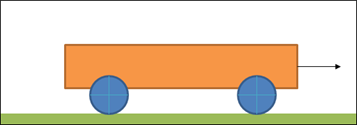
\includegraphics{Exercises/Figures/car.png}
\caption{Die zu zeichnenden Objekte}
\label{fig:car}
\end{figure}
%
\par Folgendes soll dabei gezeichnet werden:
%
\begin{itemize}
\item
Zwei Rechtecke (Orange und Grün)
\item
Zwei Kreise (Blau)
\item
Vier Linien in den Kreisen
\end{itemize}
%
\par Folgende Eigenschaften sollen animiert werden:
%
\begin{itemize}
\item
Die Position des orangen Rechtecks, der Kreise und der Linien (soll eine Fahrt
darstellen) über \jvar{dx}
\item
Der Winkel der Linien relativ zum Untergrund (soll bewegte Räder darstellen)
über \jvar{dalpha}
\end{itemize}
%
\par Sie können dies alles über Transformationen an den entsprechenden Stellen
erreichen. Für die Position sollten Sie \jfunc{translate} verwenden, für die
bewegten Räder \jfunc{rotate}. Vergessen Sie nicht die Transformationen
entsprechend zurückzusetzen.
